\chapter{Resultados experimentales y puesta en marcha}

\section{Pruebas: \textbf{\textit{desempeño}} en tarea de \textbf{\textit{clasificación}} de estafas \textbf{\textit{catfishing}} y \textbf{\textit{sextorsión}}}

En correspondencia con el objetivo del presente proyecto, se efectuó un conjunto de pruebas que involucró la creación de un \textbf{\textit{entorno}} de pruebas funcional descrito en la sección ``Pruebas de \textbf{\textit{desempeño de clasificación}} en LLMs'', en el capítulo 5 del desarrollo.

Puntualmente, esta sección concentra sus detalles en la metodología seguida para la presentación de los siguientes resultados.

En el diagrama subsecuente puede obtener una referencia visual para esclarecer los siguientes conceptos:

\begin{itemize}
    \item Las métricas descritas en el capítulo del marco teórico como ``métricas de clasificación'' se calculan para cada etiqueta contemplada; esto se debe a su naturaleza matemática, pues se establecen para evaluar problemas de clasificación binaria.
    \item Inicialmente, el problema de clasificación multietiqueta se divide o segmenta en un conjunto de pruebas binarias, una por cada etiqueta contemplada.
    \item La forma de obtener una evaluación integral que contemple el \textbf{\textit{desempeño}} del modelo para clasificar todas y cada una de las etiquetas es mediante promedios aritméticos y ponderados.
\end{itemize}

\begin{figure}[H]
    \centering
    
\includegraphics[width=1\linewidth]{imagenes/pruebas/diagramaConceptualPruebas.png}
    \caption{Diagrama conceptual sobre las métricas presentadas en la sección pruebas}
    \label{fig:diagrama-conceptual-pruebas}
\end{figure}

Considerando lo anterior, se presentan resultados mediante el promedio ponderado sobre las métricas de clasificación por cada etiqueta. De esta manera, se puede consolidar una visión general sobre el rendimiento del modelo al clasificar todas las etiquetas contempladas.

Notas: El promedio ponderado sobre la métrica F1-score resulta en la métrica unificada para observar el \textbf{\textit{desempeño}}. Considerando su definición matemática, esta se considera como la \textbf{\textit{media armónica}} que pondera las métricas precision y recall.

\subsection{Resultados con puntuación mayor a 8/10}

\begin{figure}[H]
    \centering
    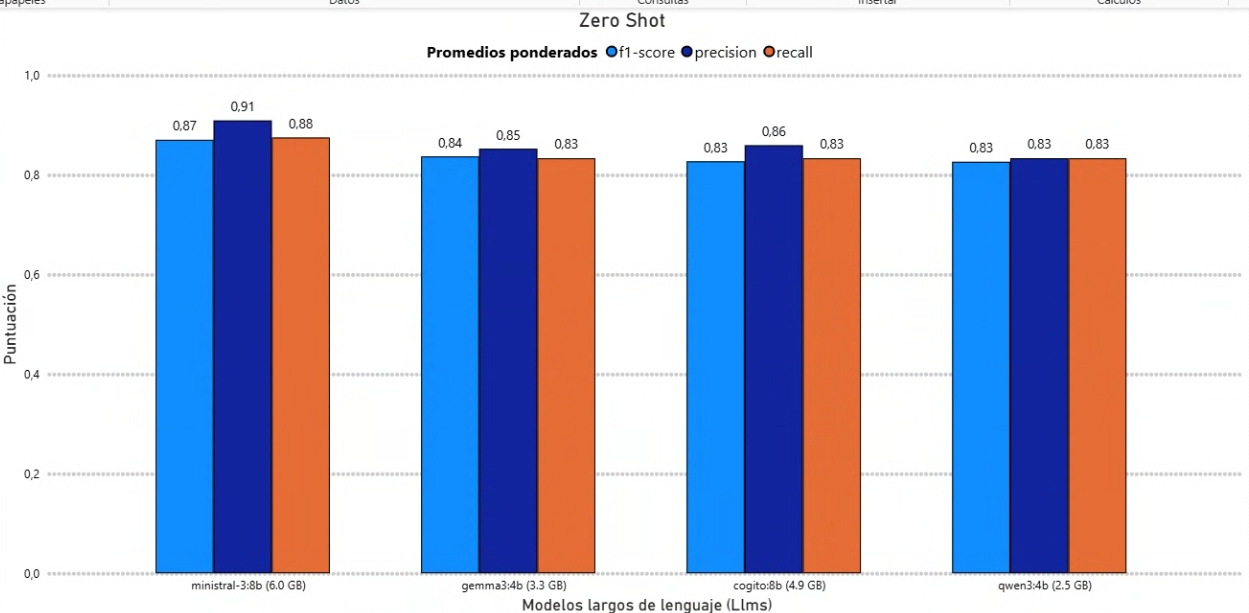
\includegraphics[width=1\linewidth]{imagenes/classificationTestsResults/Puntuacion mayor al 80/image.png}
    \caption{Modelos con puntuación mayor a 8/10 con la técnica de Zero Shot prompting}
    \label{fig:puntuacion-mayor-80-a}
\end{figure}

\begin{figure}[H]
    \centering
    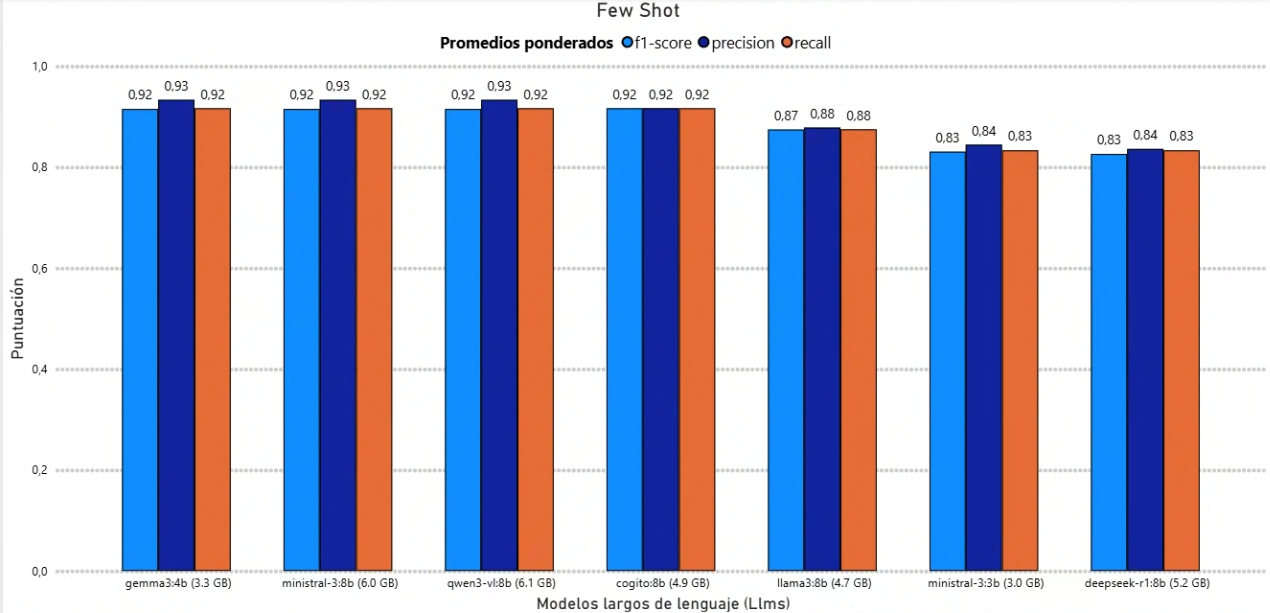
\includegraphics[width=1\linewidth]{imagenes/classificationTestsResults/Puntuacion mayor al 80/image2.png}
    \caption{Modelos con puntuación mayor a 8/10 con la técnica de Few Shot prompting}
    \label{fig:puntuacion-mayor-80-b}
\end{figure}

\subsection{Resultados con tiempo promedio por predicción menor a 4 segundos y puntuación mayor a 7/10}

\begin{figure}[H]
    \centering
    
\includegraphics[width=1\linewidth]{imagenes/classificationTestsResults/tiempo menor a 4 segundos y puntuación mayor al 70/image.png}
    \caption{Modelos con tiempo menor a 4 segundos y puntuación mayor a 7 (Zero shot)}
    \label{fig:tiempo-menor-4s-a}
\end{figure}

\begin{figure}[H]
    \centering
    
\includegraphics[width=1\linewidth]{imagenes/classificationTestsResults/tiempo menor a 4 segundos y puntuación mayor al 70/image2.png}
    \caption{Modelos con tiempo menor a 4 segundos y puntuación mayor a 7 (Few shot)}
    \label{fig:tiempo-menor-4s-b}
\end{figure}

\subsection{Resultados de puntuaciones por \textbf{\textit{escalas}} de modelos}

\begin{figure}[H]
    \centering
    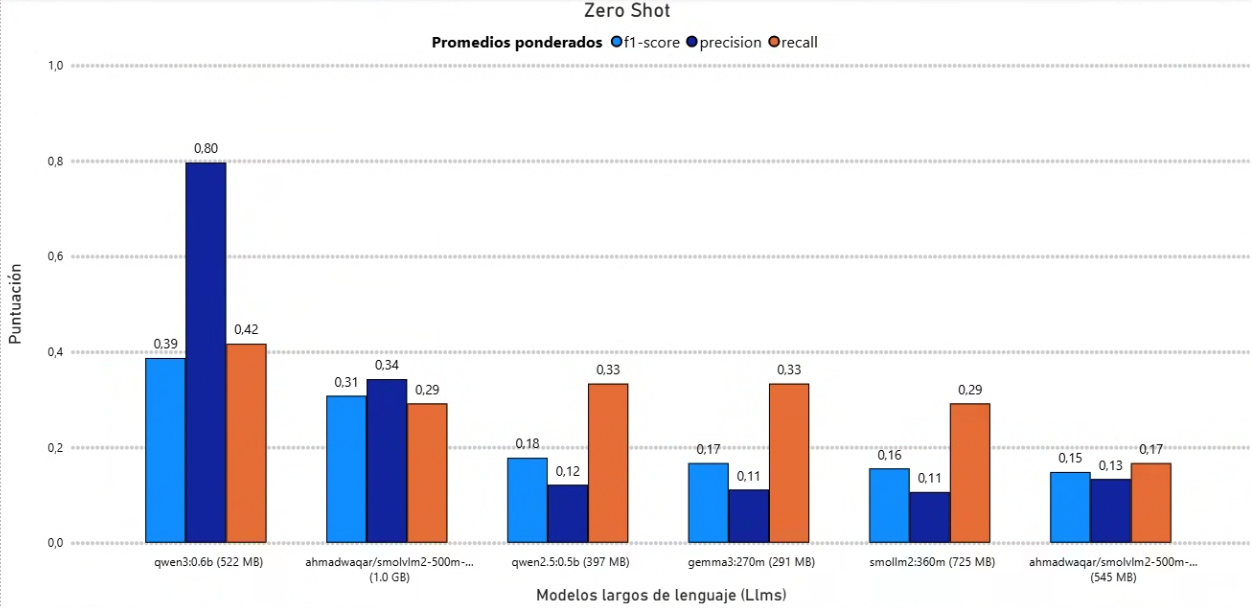
\includegraphics[width=1\linewidth]{imagenes/classificationTestsResults/modelos de 250m a 750m/zero.png}
    \caption{Resultados Zero Shot para modelos de 250m a 750m}
    \label{fig:zero-shot-250m-750m}
\end{figure}

\begin{figure}[H]
    \centering
    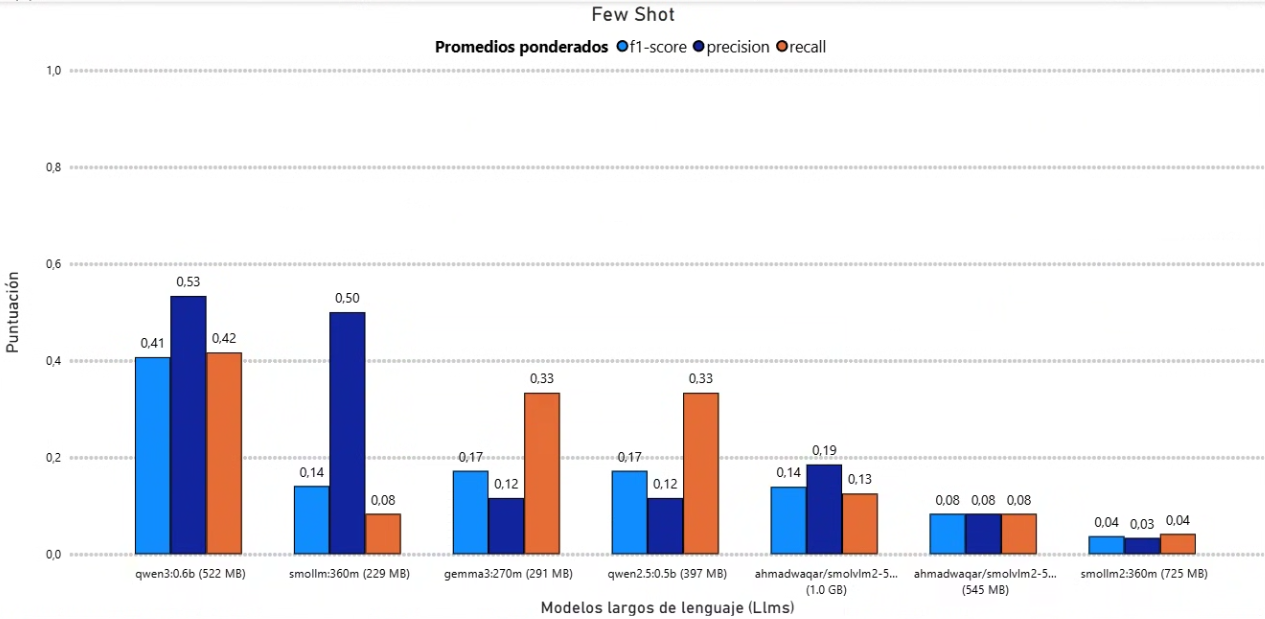
\includegraphics[width=1\linewidth]{imagenes/classificationTestsResults/modelos de 250m a 750m/few.png}
    \caption{Resultados Few Shot para modelos de 250m a 750m}
    \label{fig:few-shot-250m-750m}
\end{figure}

\begin{figure}[H]
    \centering
    
\includegraphics[width=1\linewidth]{imagenes/classificationTestsResults/modelos de 3b a 4b/zero.png}
    \caption{Resultados Zero Shot para modelos de 3b a 4b}
    \label{fig:zero-shot-3b-4b}
\end{figure}

\begin{figure}[H]
    \centering
    
\includegraphics[width=1\linewidth]{imagenes/classificationTestsResults/modelos de 3b a 4b/few.png}
    \caption{Resultados Few Shot para modelos de 3b a 4b}
    \label{fig:few-shot-3b-4b}
\end{figure}

\begin{figure}[H]
    \centering
    
\includegraphics[width=1\linewidth]{imagenes/classificationTestsResults/modelos de 7b a 8b/zero.png}
    \caption{Resultados Zero Shot para modelos de 7.75b a 8.25b}
    \label{fig:zero-shot-7b-8b}
\end{figure}

\begin{figure}[H]
    \centering
    
\includegraphics[width=1\linewidth]{imagenes/classificationTestsResults/modelos de 7b a 8b/few.png}
    \caption{Resultados Few Shot para modelos de 7.75b a 8.25b}
    \label{fig:few-shot-7b-8b}
\end{figure}
